\documentclass[11pt]{article}
\usepackage{fullpage}
\usepackage{graphicx}
\graphicspath{ {images/} }

\title{CS63 Spring 2016\\Lab 9: Unsupervised Learning}
\author{Joon Sung Park and Terry Kusunoki-Martin}

\begin{document}

\maketitle

\section{Introduction}

We chose to use the World University rankings data set.  It contained information for 2544 universities.  We used the University name as the label, and looked at 3 dimensions in particular.  We looked at the university's total score, its total number of students, and its student/faculty ratio.  

the data can be found here at https://www.kaggle.com/mylesoneill/world-university-rankings

\section{Analysis}

Describe the results of applying both hierarchical clustering and
k-means.  For hierarchical clustering, give examples of interesting
clusters found.  Show a picture of the resulting tree.  For k-means,
how did you choose k?  What was the best error found?  Which approach
seems to better fit your data? Why?
\begin{center}
 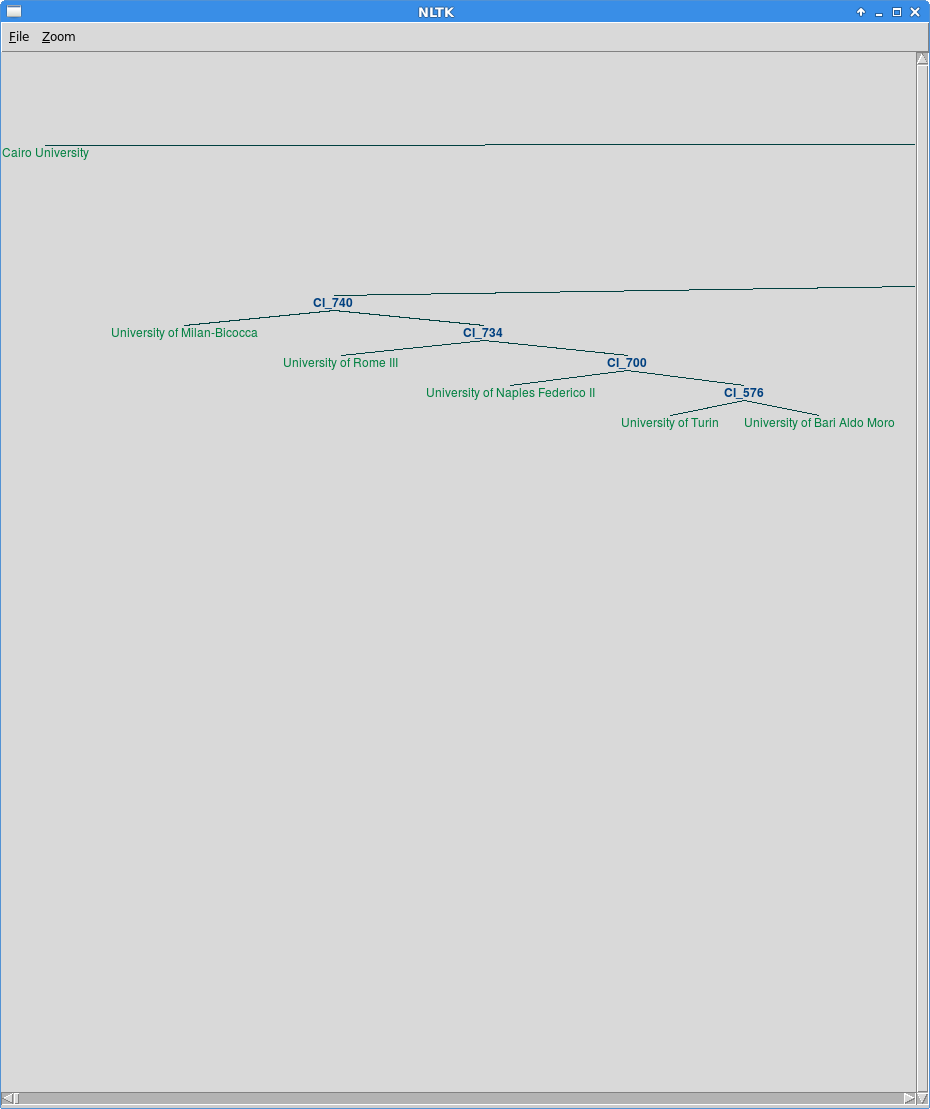
\includegraphics[scale=0.5]{hierarchical}
 \\ 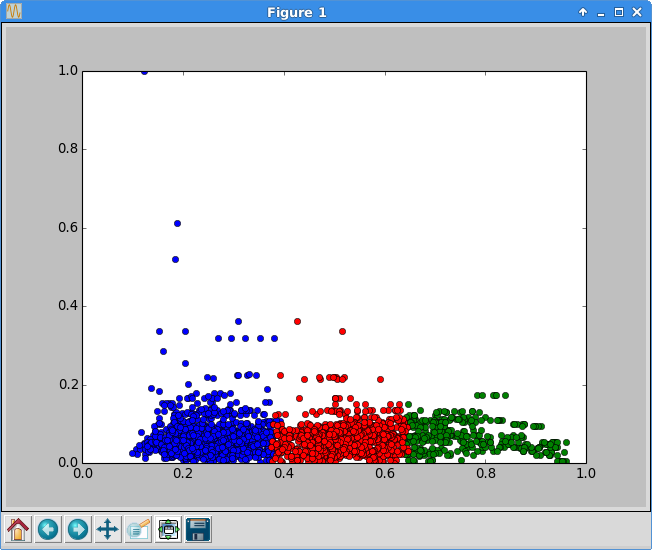
\includegraphics[scale=0.7]{kmeans}
\end{center}
The hierarchical clustering was hard to parse since the tree was so large.  However, observing a subtree such as this shows that the universities beibng clustered together using the dimensions we chose roughly aligned with the university rankings.  All the universities in this subtree pictured above are tied for 350-400 in the university ranking list.\\

The kmeans clustering required us to normalize the data so that the points would fit in the window.  We achieved this by looking for the max value of each dimension and dividing all values by the average for that dimension.  The kmeans plot is plotting total score along the x axis and number of students along the y axis.  As we would suspect, the higher the score goes the lower the average number of students is.  We chose k=3 because there were 3 dimensions, and it turned out that this allowed the clustering to complete the fastest.  The lowest error found was 0.05.  Kmeans doesn't seem to make sense to use here.  The data is harder to parse (or at least harder to visualize) because we can't look at the university names for each data point.  Hierarchical clustering allows us to clearly see that closely ranked universities are clustered together.

\section{Conclusion}

We cound that universities with similar numbers of students and student/faculty ratio also rank similar on the world university rankings list.  This is something that we intuit with the way we talk about universities colloquially, and these clustering algorithms support our intuitions.

\end{document}
